\documentclass[twocolumn,showpacs,amsmath,amssymb]{revtex4}

\usepackage{graphicx}   % Include figure files
\usepackage{dcolumn}   % Align table columns on decimal point
\usepackage{bm}            % bold math
\usepackage{subfig}

% Johnston-Doering custom commands
\newcommand{\R}{\mbox{R}}
\newcommand{\Rhat}{\hat{\mbox{R}}}
\newcommand{\Ra}{\mbox{Ra}}
\newcommand{\Nu}{\mbox{Nu}}
\newcommand{\Pran}{\mbox{Pr}}

\def\DN{\mathcal{D}_N}
\def\tilde{\widetilde}
\def\hat{\widehat}
\def\lap{\Delta}
\def\bar{\overline}
\def\del{\partial}
\def\DOT{\!\cdot\!}
\def\dt{{\Delta t}} 
\def\dx{{\Delta x}}
\def\dy{{\Delta y}}
\def\u{\mbox{\boldmath $u$}}
\def\n{\mbox{\boldmath $n$}}
\def\f{\mbox{\boldmath $f$}}
\def\Circ{{\footnotesize$\bigcirc$}}
\def\Bullet{{\large$\bullet$}}

\newcommand{\qref}[1]{(\ref{#1})} 
\newcommand{\khat}{{\bf \hat{k}}}
\newcommand{\jhat}{{\bf \hat{j}}}
\newcommand{\ihat}{{\bf \hat{i}}}

\begin{document}

\title{Marginally-Stable Thermal Equilibria of Rayleigh Benard Convection}

\author{Sharrod Brown}
\affiliation{%
Senator (D), Ohio}

% \author{Daniel Lecoanet}
% \affiliation{%
% Physics Department, University of California, Berkeley, CA 94720, USA\\
% Astronomy Department and Theoretical Astrophysics Center, University of California, Berkeley, CA 94720, USA\\
% Princeton Center for Theoretical Science, Princeton University, Princeton, NJ 08544, USA\\
% Department of Astrophysical Sciences, Princeton University, Princeton, NJ 08544, USA\\
% Kavli Institute for Theoretical Physics, University of California, Santa Barbara, CA 93106, USA}

% \author{Rich R. Kerswell}
% \affiliation{%
% DAMTP, Centre for Mathematical Sciences, Cambridge University, Cambridge CB3 0WA, UK \\
% School of Mathematics, University of Bristol, Bristol BS8 1TW, UK\\
% Kavli Institute for Theoretical Physics, University of California, Santa Barbara, CA 93106, USA}
% \date{\today}% It is always \today, today,
%              %  but any date may be explicitly specified


\begin{abstract}

Sometimes your professor will ask you to include an abstract, or general summary of your work, with your research paper. The abstract allows you to elaborate upon each major aspect of the paper and helps readers decide whether they want to read the rest of the paper. Therefore, enough key information [e.g., summary results, observations, trends, etc.] must be included to make the abstract useful to someone who may want to examine your work.

How do you know when you have enough information in your abstract? A simple rule-of-thumb is to imagine that you are another researcher doing a similar study. Then ask yourself: if your abstract was the only part of the paper you could access, would you be happy with the amount of information presented there? Does it tell the whole story about your study? If the answer is "no" then the abstract likely needs to be revised.

\end{abstract}


\maketitle

\section{Introduction}

The introduction leads the reader from a general subject area to a particular topic of inquiry. It establishes the scope, context, and significance of the research being conducted by summarizing current understanding and background information about the topic, stating the purpose of the work in the form of the research problem supported by a hypothesis or a set of questions, explaining briefly the methodological approach used to examine the research problem, highlighting the potential outcomes your study can reveal, and outlining the remaining structure and organization of the paper.

% \section{Procedures}\label{sec:procedures}
\section{Conventional Boussinesq Linear Stability Analysis}\label{sec:boussinesq}
We begin with the non-dimensionalized Boussinesq approximation for Rayleigh-Bénard Convection. The domain is 2-dimensional rectangular with spatial dimensions $x$ and $z$ where $0 < x < 4$ and $-1/2 < z < 1/2$. The fluid is constrained between two planar boundaries at $z = -1/2$ and $z = 1/2$ with fixed temperatures $1$ and $0$ respectively. At both boundaries we specify impenetrable and no-slip conditions, such that the velocity $\mathbf{u} = u \hat{x} + w \hat{z} = \mathbf{0}$ at $z = \pm 1/2$. The domain is periodic in the horizontal direction. The equations of motion are then given by
\begin{align}
    \nabla \cdot \mathbf{u} &= 0 \label{EQ:motion1}\\
    \frac{\partial \mathbf{u}}{\partial t} + \mathbf{u} \cdot \nabla \mathbf{u} &= - \nabla p + T \hat{z} + \sqrt{\frac{Pr}{Ra}} \nabla^2 \mathbf{u} \label{EQ:motion2}\\
    \frac{\partial T}{\partial t} + \mathbf{u} \cdot \nabla T &= \frac{1}{\sqrt{RaPr}} \nabla^2 T \label{EQ:motion3}
\end{align}
where $p$ is pressure and $T$ is temperature. For completeness, we specify a final boundary condition $p = p_0$ at $z = \pm 1/2$. Any system of this form can be characterized by its Rayleigh number $Ra$ and Prandtl number $Pr$, where $Ra$ is the timescale ratio of thermal diffusion to convection and $Pr$ is the ratio of momentum diffusivity to thermal diffusivity.  For convenience, we define 
\begin{equation}
\mathcal{R} = \sqrt{\frac{Pr}{Ra}}, \qquad \mathcal{P} = \frac{1}{\sqrt{Pr Ra}}
\end{equation}
\par To derive the linearized system, we posit that each field can be represented as the sum of a background profile (denoted by $\bar{\cdot } \;$) and a perturbation function (denoted by $\cdot'$). Suppose $\frac{\partial \bar{T}}{\partial z}\big|_{t=t_0} (z)$ is some given function which satisfies
\begin{equation}
    \int_{-\frac{1}{2}}^{\frac{1}{2}} \frac{\partial \bar{T}}{\partial z}\Big|_{t=t_0} dz = -1
\end{equation}
then the background profiles are given by
\begin{align}
    \mathbf{\bar{u}} &= \mathbf{0} \\
    \bar{T}(z) &= 1 + \int_{-\frac{1}{2}}^{z} \frac{\partial \bar{T}}{\partial \zeta}\Big|_{t=t_0}(\zeta) d\zeta \\
    \bar{p}(z) &= p_0 - \int_{-\frac{1}{2}}^z \bar{T}(\zeta) d\zeta
\end{align}
Accordingly, we rewrite the fields as
\begin{align}
    \mathbf{u}(x, z, t) &= \mathbf{u'}(x, z, t) \label{EQ:reynolds_dc_u}\\
    &= u'(x, z, t)\hat{x} + w'(x, z, t)\hat{z} \\
    T(x, z, t) &= \bar{T}(z) + T'(x, z, t) \label{EQ:reynolds_dc_T}\\
    p(x, z, t) &= \bar{p}(z) + p'(x, z, t)
\end{align}
Upon substitution, we equate terms which scale linearly with the perturbations, yielding the following linearized stability equations
\begin{align}
    \nabla \cdot \mathbf{u'} &= 0 \label{EQ:linear1}\\
    \frac{\partial\mathbf{u'}}{\partial t} &= - \nabla p' + T'\hat{z} + \mathcal{R} \nabla^2 \mathbf{u'} \label{EQ:linear2}\\
    \frac{\partial T'}{\partial t} + \frac{\partial \bar{T}}{\partial z} w' &= \mathcal{P} \nabla^2 T'\label{EQ:linear3}
\end{align}
With Dirichlet boundary conditions 
\begin{equation}
    T'|_{z = \pm \frac{1}{2}} = 0, \quad u'|_{z = \pm \frac{1}{2}} = 0, \quad p'|_{z = \pm \frac{1}{2}} = 0
\end{equation}
In 1916, Lord Rayleigh observed that (\ref{EQ:linear1}) and (\ref{EQ:linear3}) can be manipulated into a separable form with generalized solutions
\begin{align}
    w'(x, z, t) &= W(z) \, e^{i(k_xx-st)} \label{EQ:normal_modes1}\\ 
    u'(x, z, t) &= U(z) \, e^{i(k_xx-st)} \label{EQ:normal_modes2}\\ 
    T'(x, z, t) &= \Theta(z) \, e^{i(k_xx-st)} \label{EQ:normal_modes3}\\ 
    p'(x, z, t) &= P(z) \, e^{i(k_xx-st)}\label{EQ:normal_modes4}
\end{align}
where $s = \sigma + i\omega$ and $k_x$ is restricted by periodicity to the countably infinite set (spectrum) of wavenumbers
\begin{align}
    k_x \in \big\{\frac{n\pi}{2} \, \big| \, n \in \mathbb{N}\big\}
\end{align}
For each $k_x$, we can assess the stability of the perturbations by solving for the eigenvalue $s$, whose imaginary component $\omega$ plays the role of an exponential growth rate. Solution generally yields a finite set of eigenvalues, among which, that with the maximum value of $\omega$ is assumed to be dominant. Positive eigenvalues indicate that the system is unstable to small disturbances of wavenumber $k_x$, while negative eigenvalues indicate stability. A complete linear stability analysis requires that we solve over the full spectrum of wavenumbers. The prototypical case is used to demonstrate that the critical Rayleigh number $Ra_c = 1708$ when $\frac{\partial \bar{T}}{\partial z}\big|_{t=t_0} = -1$.

\section{Temperature profile evolution}\label{sec:evolution}
For this investigation, we allow $ \bar{T}$ to vary in $z$ and $t$. Substituting (\ref{EQ:reynolds_dc_T}) into (\ref{EQ:motion3}) yields
\begin{align}
    \frac{\partial \bar{T}}{\partial t} + \mathbf{u}' \cdot \nabla T' + \frac{\partial T'}{\partial t} + \frac{\partial \bar{T}}{\partial z} w' = \mathcal{P} \nabla^2 T' + \mathcal{P} \nabla^2 \bar{T}.
    \label{EQ:T't_xz}
\end{align}
Subtracting (\ref{EQ:linear3}) from (\ref{EQ:T't_xz}) eliminates several terms. We can also replace the advective term $\mathbf{u}' \cdot \nabla T'$ with $\grad \cdot (\mathbf{u}'T')$ due to (\ref{EQ:linear1}). By taking the horizontal average of (\ref{EQ:T't_xz}), this advective term can be reduced to
\begin{align}
    \frac{1}{4}\int_0^4 \grad \cdot (\mathbf{u}'T') dx &= \frac{\partial }{\partial z}  \langle w'T' \rangle
\end{align}
where $\langle \cdot \rangle$ denotes the horizontal average. The remaining terms in (\ref{EQ:T't_xz}) are unaffected as they are independent of $x$. Lastly, it is important to note that the eigenfunctions do not admit any natural normalization, as (\ref{EQ:linear1}) - (\ref{EQ:linear3}) and their subsequent forms are linear with respect to the perturbations. For completeness, we provide the normalization 
\begin{equation}
    \int_{-\frac{1}{2}}^{\frac{1}{2}} \big| \Theta (z) \big| dz = 1
\end{equation}
and assign each perturbation a yet-unknown amplitude $A \in \mathbb{R}$, thereby allowing us to rewrite (\ref{EQ:T't_xz}) as an initial value problem (IVP)
\begin{equation}
    \frac{\partial \bar{T}}{\partial t} + A^2 \langle w'T' \rangle = \mathcal{P}  \frac{\partial^2 \bar{T}}{\partial z^2} \label{EQ:T0_IVP}
\end{equation}
which can be characterized as a nonhomogeneous  1-dimensional diffusion equation, upon which the rest of this investigation is focused. It is important to keep in mind that the forcing term $\langle w'T' \rangle$ is obtained by solving an eigenvalue problem (EVP) which itself involves $\frac{\partial \bar{T}}{\partial z}$. More specifically, we assume that stable modes do not affect the evolution of $\bar{T}$.
\par For various Rayleigh numbers and fixed $Pr = 1$, we seek symmetric, marginally-stable temperature profiles $\bar{T}_{eq}(z)$ which are thermally equilibrated, thereby satisfying $\frac{\partial \bar{T}_{eq}}{\partial t} = 0$, according to (\ref{EQ:T0_IVP}). We employ the \texttt{Dedalus} pseudo-spectral python framework to solve the EVP outlined in Section \ref{sec:boussinesq} as well as the IVP (\ref{EQ:T0_IVP}) by representing each field with a dealiased Chebshev Polynomial basis. The required number of basis functions varies, as Temperature profiles associated with higher Rayleigh numbers demand increasingly small-scale structures to resolve their aggressive boundary layers. We supplement \texttt{Dedalus} with the \texttt{Eigentools} package to obtain the eigenfunctions included in (\ref{EQ:T0_IVP}).
\par To find an equilibrated profile, we begin with a marginally-stable initial profile $\bar{T}_0(z)$ which is constructed as described in \ref{sec:initial_profile}. We seek to evolve $\bar{T}_0(z)$ into a new marginally-stable profile $\bar{T}_1(z)$ according to (\ref{EQ:T0_IVP}) by using forward-Euler. This generally requires a unique and unknown value $A^2 > 0$. Our method of finding $A^2$ is best illustrated through example.

\begin{figure}[h]
    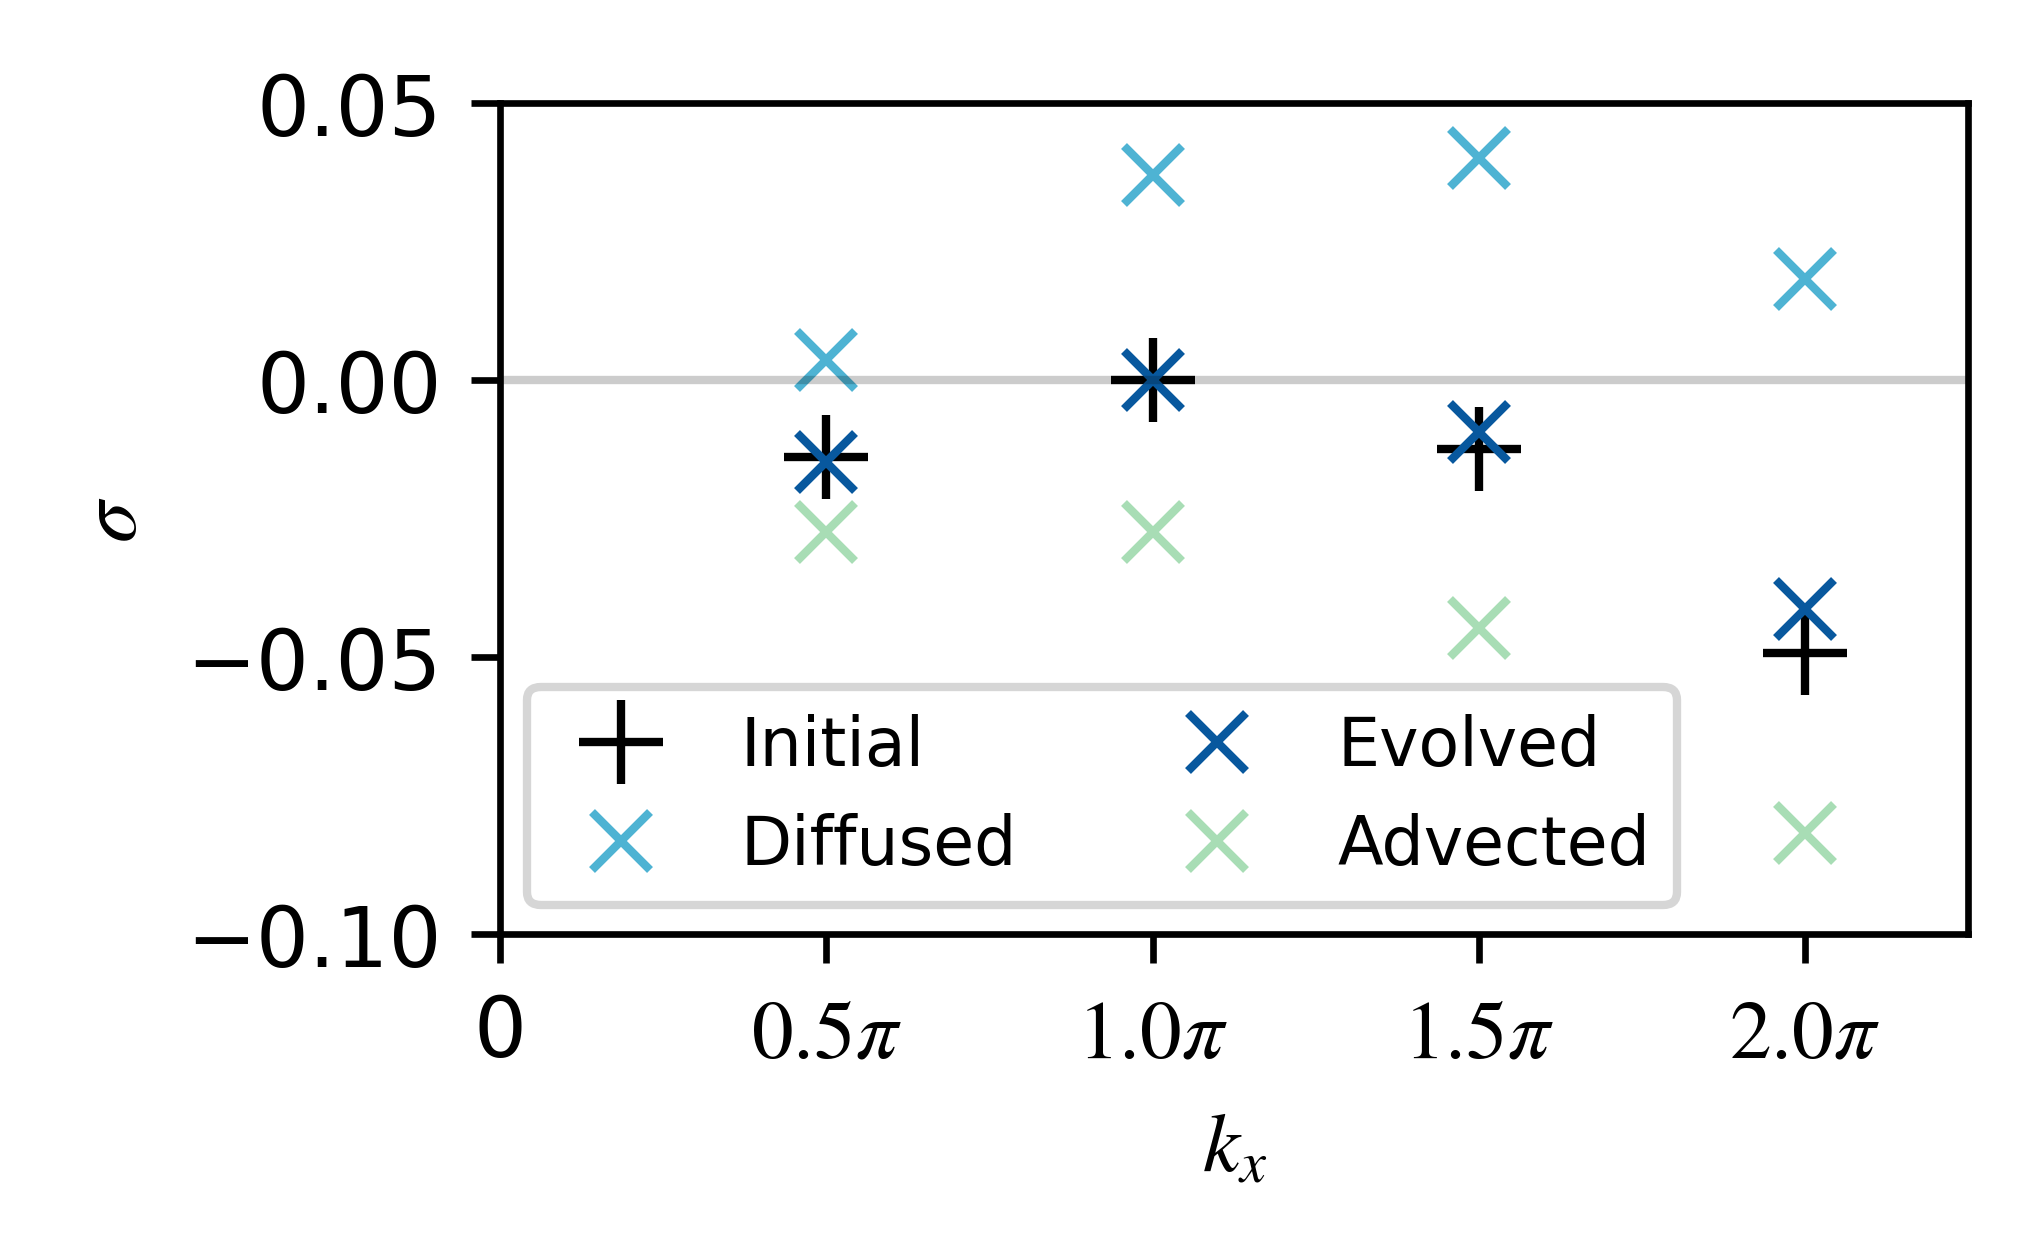
\includegraphics[width=3.4in]{EV_spectrum_ol.png}
    \caption{Eigenvalue spectra for $Ra = 10^5$. The spectrum of a marginally-stable background temperature profile $\bar{T}_0$ has a maximum eigenvalue of 0. Given a small constant timestep $\Delta t$, diffusion destabilizes the system, increasing its eigenvalues. Advection tends to stabilize the system, decreasing its eigenvalues. It follows that there exists some proportion ($A^2$) of these two terms which yields a new marginally-stable background temperature profile $\bar{T}_1$ when the original profile $\bar{T}_0$ is evolved according to (\ref{EQ:T0_IVP}).}
    \label{fig:iteration_spectra} 
\end{figure}

In Figure \ref{fig:iteration_spectra} we perform an iteration as follows: diffusing a marginally-stable temperature profile $\bar{T}_0$ tends to increase its eigenvalues. Ignoring the diffusive term and evolving according to advection tends the stabilize the system. The appropriate amplitude $A^2$ can then be approximated by
\begin{equation}
    A^2 \sim -\frac{\omega_{diff}}{\omega_{adv}}
\end{equation}
where $\omega_{diff}$ and $\omega_{adv}$ refer to the diffused and advected eigenvalues of the initially marginally-stable mode respectively. $\bar{T}_0$ is then evolved according to (\ref{EQ:T0_IVP}), after which another eigenvalue solve is performed on the evolve temperture profile. Given a fixed timestep $\Delta t$, we assume the dominant eigenvalue can be described by a smooth function $\omega (A^2) = \max \{ \omega_{kx} \}$. We then employ Newton's method to find the appropriate amplitude by approximating $\omega'(A^2)$ with 1st-order finite-differences and specifying a tolerance $1e-9$. The dominant mode is not fixed; an iteration can facilitate the transfer of marginal stability from one mode to another. In section \ref{sec:multiple_modes} we specify procedures for the treatment of multiple simultaneously marginal modes.
% How does the EV spectrum respond to diffusion (amplitudes are zero)? This is likely due to growth in the boundary layer height. How does it respond to advective fluxes of differing wavenumbers (amplitudes are large). Point out that the amplitude is not constrained mathematically (but it must be nonnegative!), then use the fact that the new state must be marginally-stable to find the appropriate amplitude(s).
% \begin{figure}[H]
%     \centering
%     \includegraphics[width=3.4in]{b0_evolution.PNG}
%     \caption{b0z over several iterations}
%     \label{fig:b0z_iterations}
% \end{figure}
% We can do the same with the horizontal momentum equation but in this case we seek symmetrical solutions, implying the mean horizontal flow is zero. More investigation is needed for systems with flux-temperature boundary conditions or asymmetrical solutions in general. Show b0z evolution fig? 
\subsection{Initial buoyancy profile} \label{sec:initial_profile}
In an attempt to minimize the required number of iterations, we employ the analytical thermal boundary layer equation for turbulent Rayleigh-Benard convection given by \ref{ref:BL_EQs}
\begin{align}
    \bar{T}_0(\xi) &= \frac{\sqrt{3}}{4\pi} \log \frac{(1 + a\xi)^3}{1 + (a\xi)^3} + \frac{3}{2\pi} \arctan \Big( \frac{4\pi}{9}\xi - \frac{1}{\sqrt{3}} \Big) + \frac{1}{4} \nonumber \\
    \xi &= \frac{z}{\delta_0}, \qquad a = \frac{2\pi}{3\sqrt{3}}\label{EQ:T0}
\end{align}
where $\delta_0$ is the boundary layer thickness. Anticipating $Ra \sim \delta^{-3}_0$, we expect that each $\Ra$ is associated with a unique $\delta_0$ for which $\bar{T}_0(z)$ is marginally stable. It should be noted that while experimenting with different initial profiles, we still obtain congruent equilibrated profiles $\bar{T}_{eq}(z)$, suggesting that these states may be unique. An example of (\ref{EQ:T0}) is shown in Figure \ref{fig:b0z_iterations}.

% \begin{figure}[h]
%     \centering
%     \includegraphics[width=3.4in]{QG0.png}
%     \caption{Kx marginals vs sim time or iteration}
%     \label{fig:my_label}
% \end{figure}

\subsection{Treatment of multiple marginally-stable modes} \label{sec:multiple_modes}
In most cases, we eventually encounter eigenvalue spectra with multiple marginally stable modes. If ignored, we are forced to reduce the timestep and allow the modes to alternate. Instead, we generalize the advective term in (\ref{EQ:T0_IVP}) to accommodate $N$ simultaneously marginal modes
\begin{equation}
    A^2 \langle w' b' \rangle = \sum_{n = 1}^{N} A^2_{n} \langle w' b' \rangle_{n}
\end{equation}
where  $\langle w' b' \rangle_{n}$ is composed of eigenfunctions associated with $k_x = \frac{n\pi}{2}$. There are now $N$ amplitudes to solve for and $N$ eigenvalues to keep marginally stable. In general, we expect a function $\mathbf{\omega} \, : \, \mathbb{R}^N \to  \mathbb{R}^N$ to have isolated roots (should they exist). We employ Broyden's method for root-finding in multiple dimensions with discretized data. The difficulty arises when transitioning between different numbers of marginal modes. Here we rely on $A^2 > 0$ by asserting that a mode which is \textit{close enough} to marginal stability can be included in the iteration provided that its respective amplitude is positive. Should we converge upon a negative amplitude, that mode is discarded and the iteration is repeated. In general we find that any other course of action fails to equilibrate.
\newline
% \begin{figure}[t]
%     \centering
%     \includegraphics[width=3.1in]{EV_spectrum_lapse2.png}
%     \caption{Marginally stable eigenvalue spectra: $Ra = 2e9$}
%     \label{fig:spectra_lapse}
% \end{figure}
\section{Properties of Thermally Equilibrated States}\label{sec:properties}
Thermally equilibrated states of this kind are solutions to the quasilinear Rayleigh Benard convection equations. For this investigation, we calculate solutions for Rayleigh numbers in the range $10^5 - 10^9$. Thermal equilibrium is synonymous with constant heat flux by (\ref{EQ:T0_IVP}). Solutions are symmetric about $z = 0$ by design. This, combined with the fact that we did initialize a background horizontal flow implies the absence of any nonconstant horizontal flow perturbations. 
\par In general, marginally-stable thermal equilibria can be characterized by their boundary layer thicknesses, from which, the rest of their properties follow. Letting the interior boundary layer threshold be the $z$-coordinate at which $\frac{\partial \bar{T}}{\partial z} = 0$, we find that $Ra \propto  \delta^{-3}$ as illustrated in Figure \ref{fig:bl_ra}. This is consistent with Malkus' marginal stability theory, a scaling argument which perceives the boundary regions as subdomains which are themselves marginally stable \ref{source:Malkus?}.

\begin{figure}[h]
    \centering
    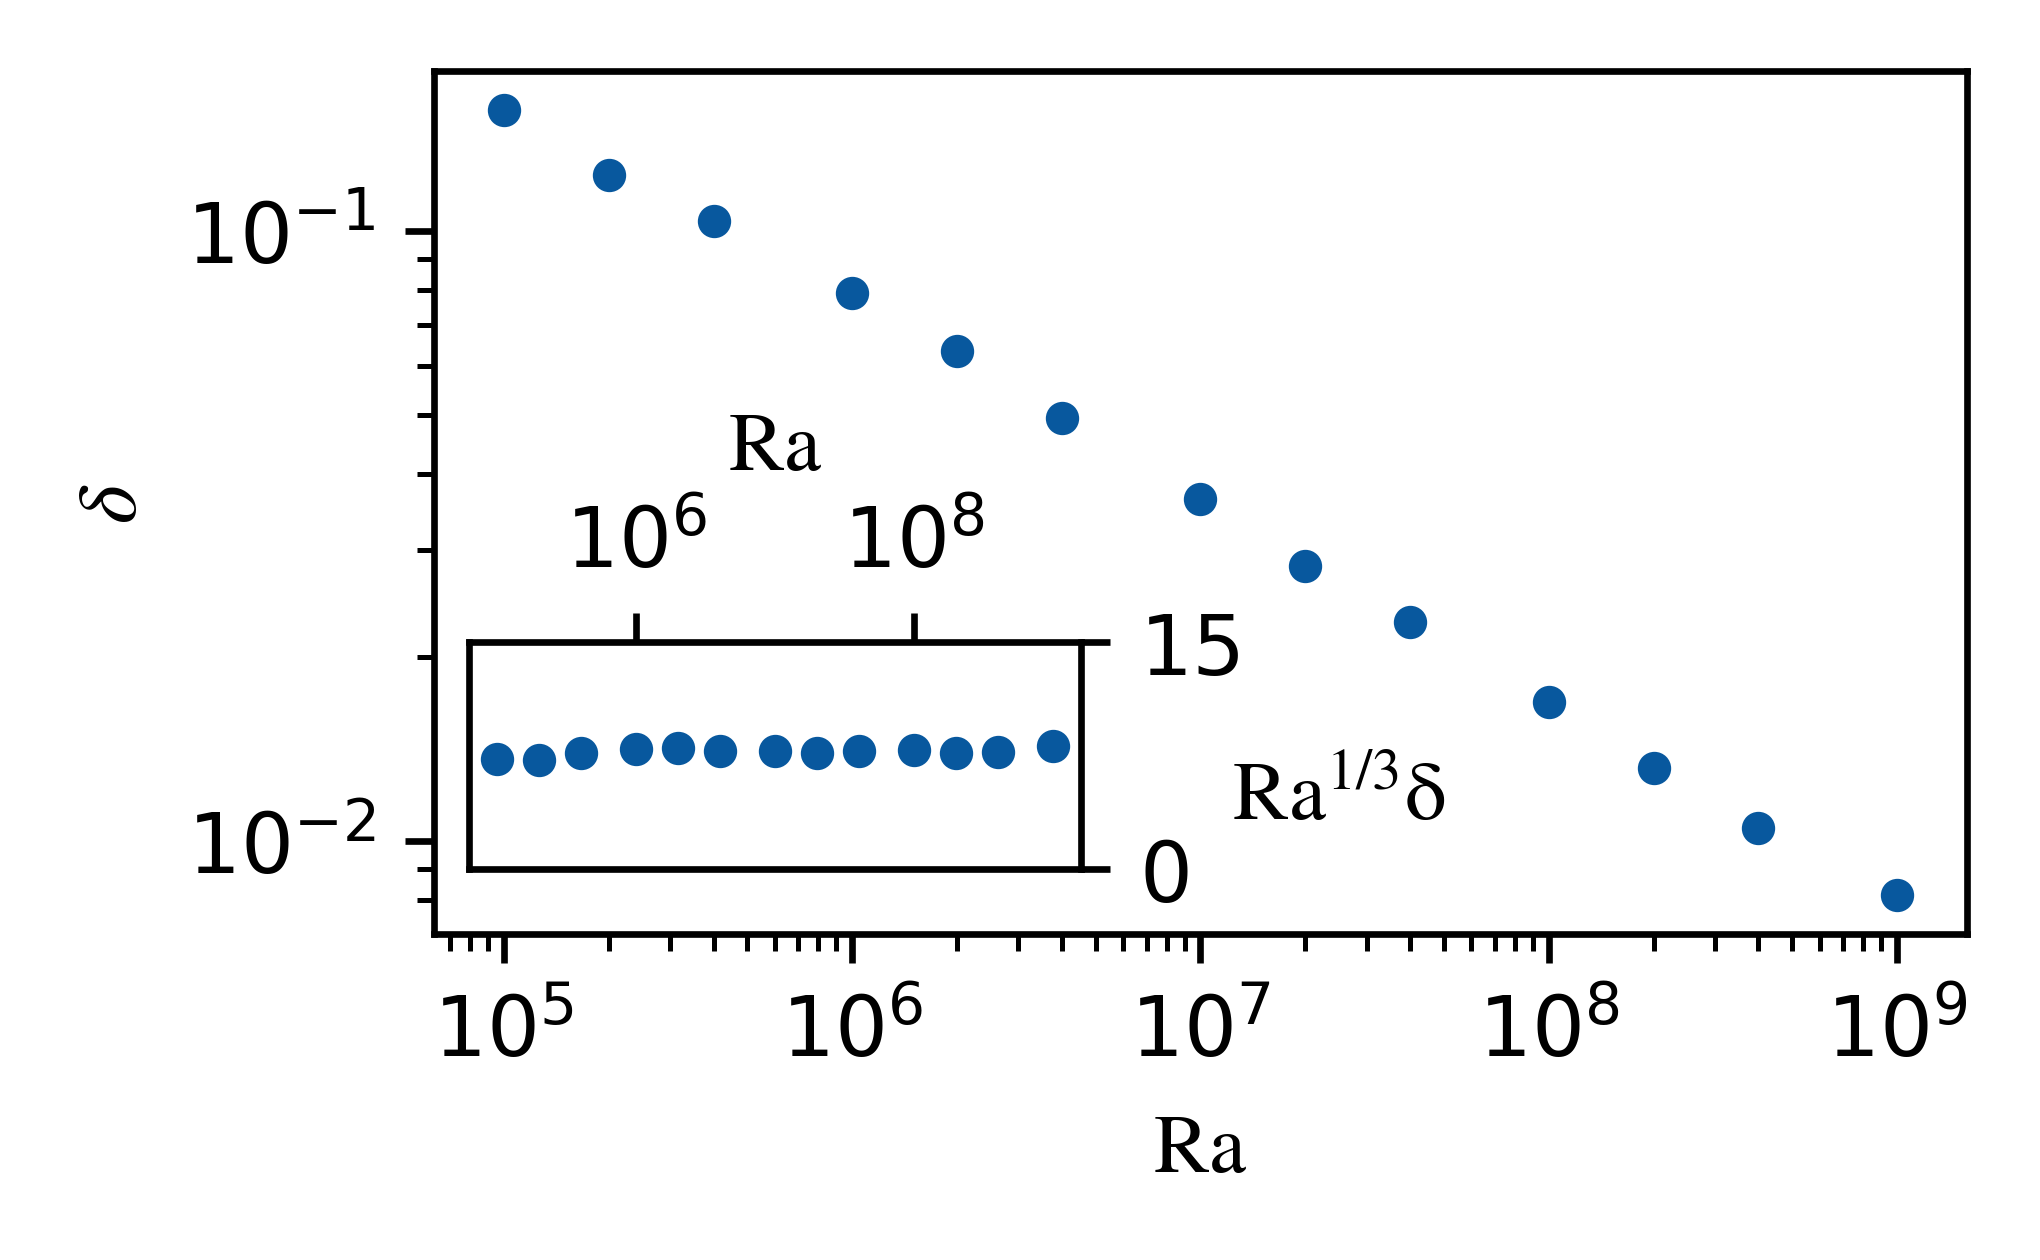
\includegraphics[width=3.4in]{del_ra.PNG}
    \caption{Boundary layer widths $\delta$ of marginally-stable thermal equilibria. We define the threshold of each boundary layer as the $z$-coordinate at which $\frac{\partial \bar{T}}{\partial z} = 0$, corresponding to the local extrema of the ``Thermally Equilibrated" curve in Figure \ref{fig:T0_profiles}. Plotting on a log-log scale, we find that $\delta$ and $Ra$ obey a power-law relationship. We also demonstrate that $Ra^{1/3}\delta$ is approximately constant with respect to $Ra$ implying $Ra \propto  \delta^{-3}$, as predicted by \ref{source:???} (scaling arguments literature)}
    \label{fig:bl_ra}
\end{figure}

\begin{figure*}[t]
    \centering
    \subfloat{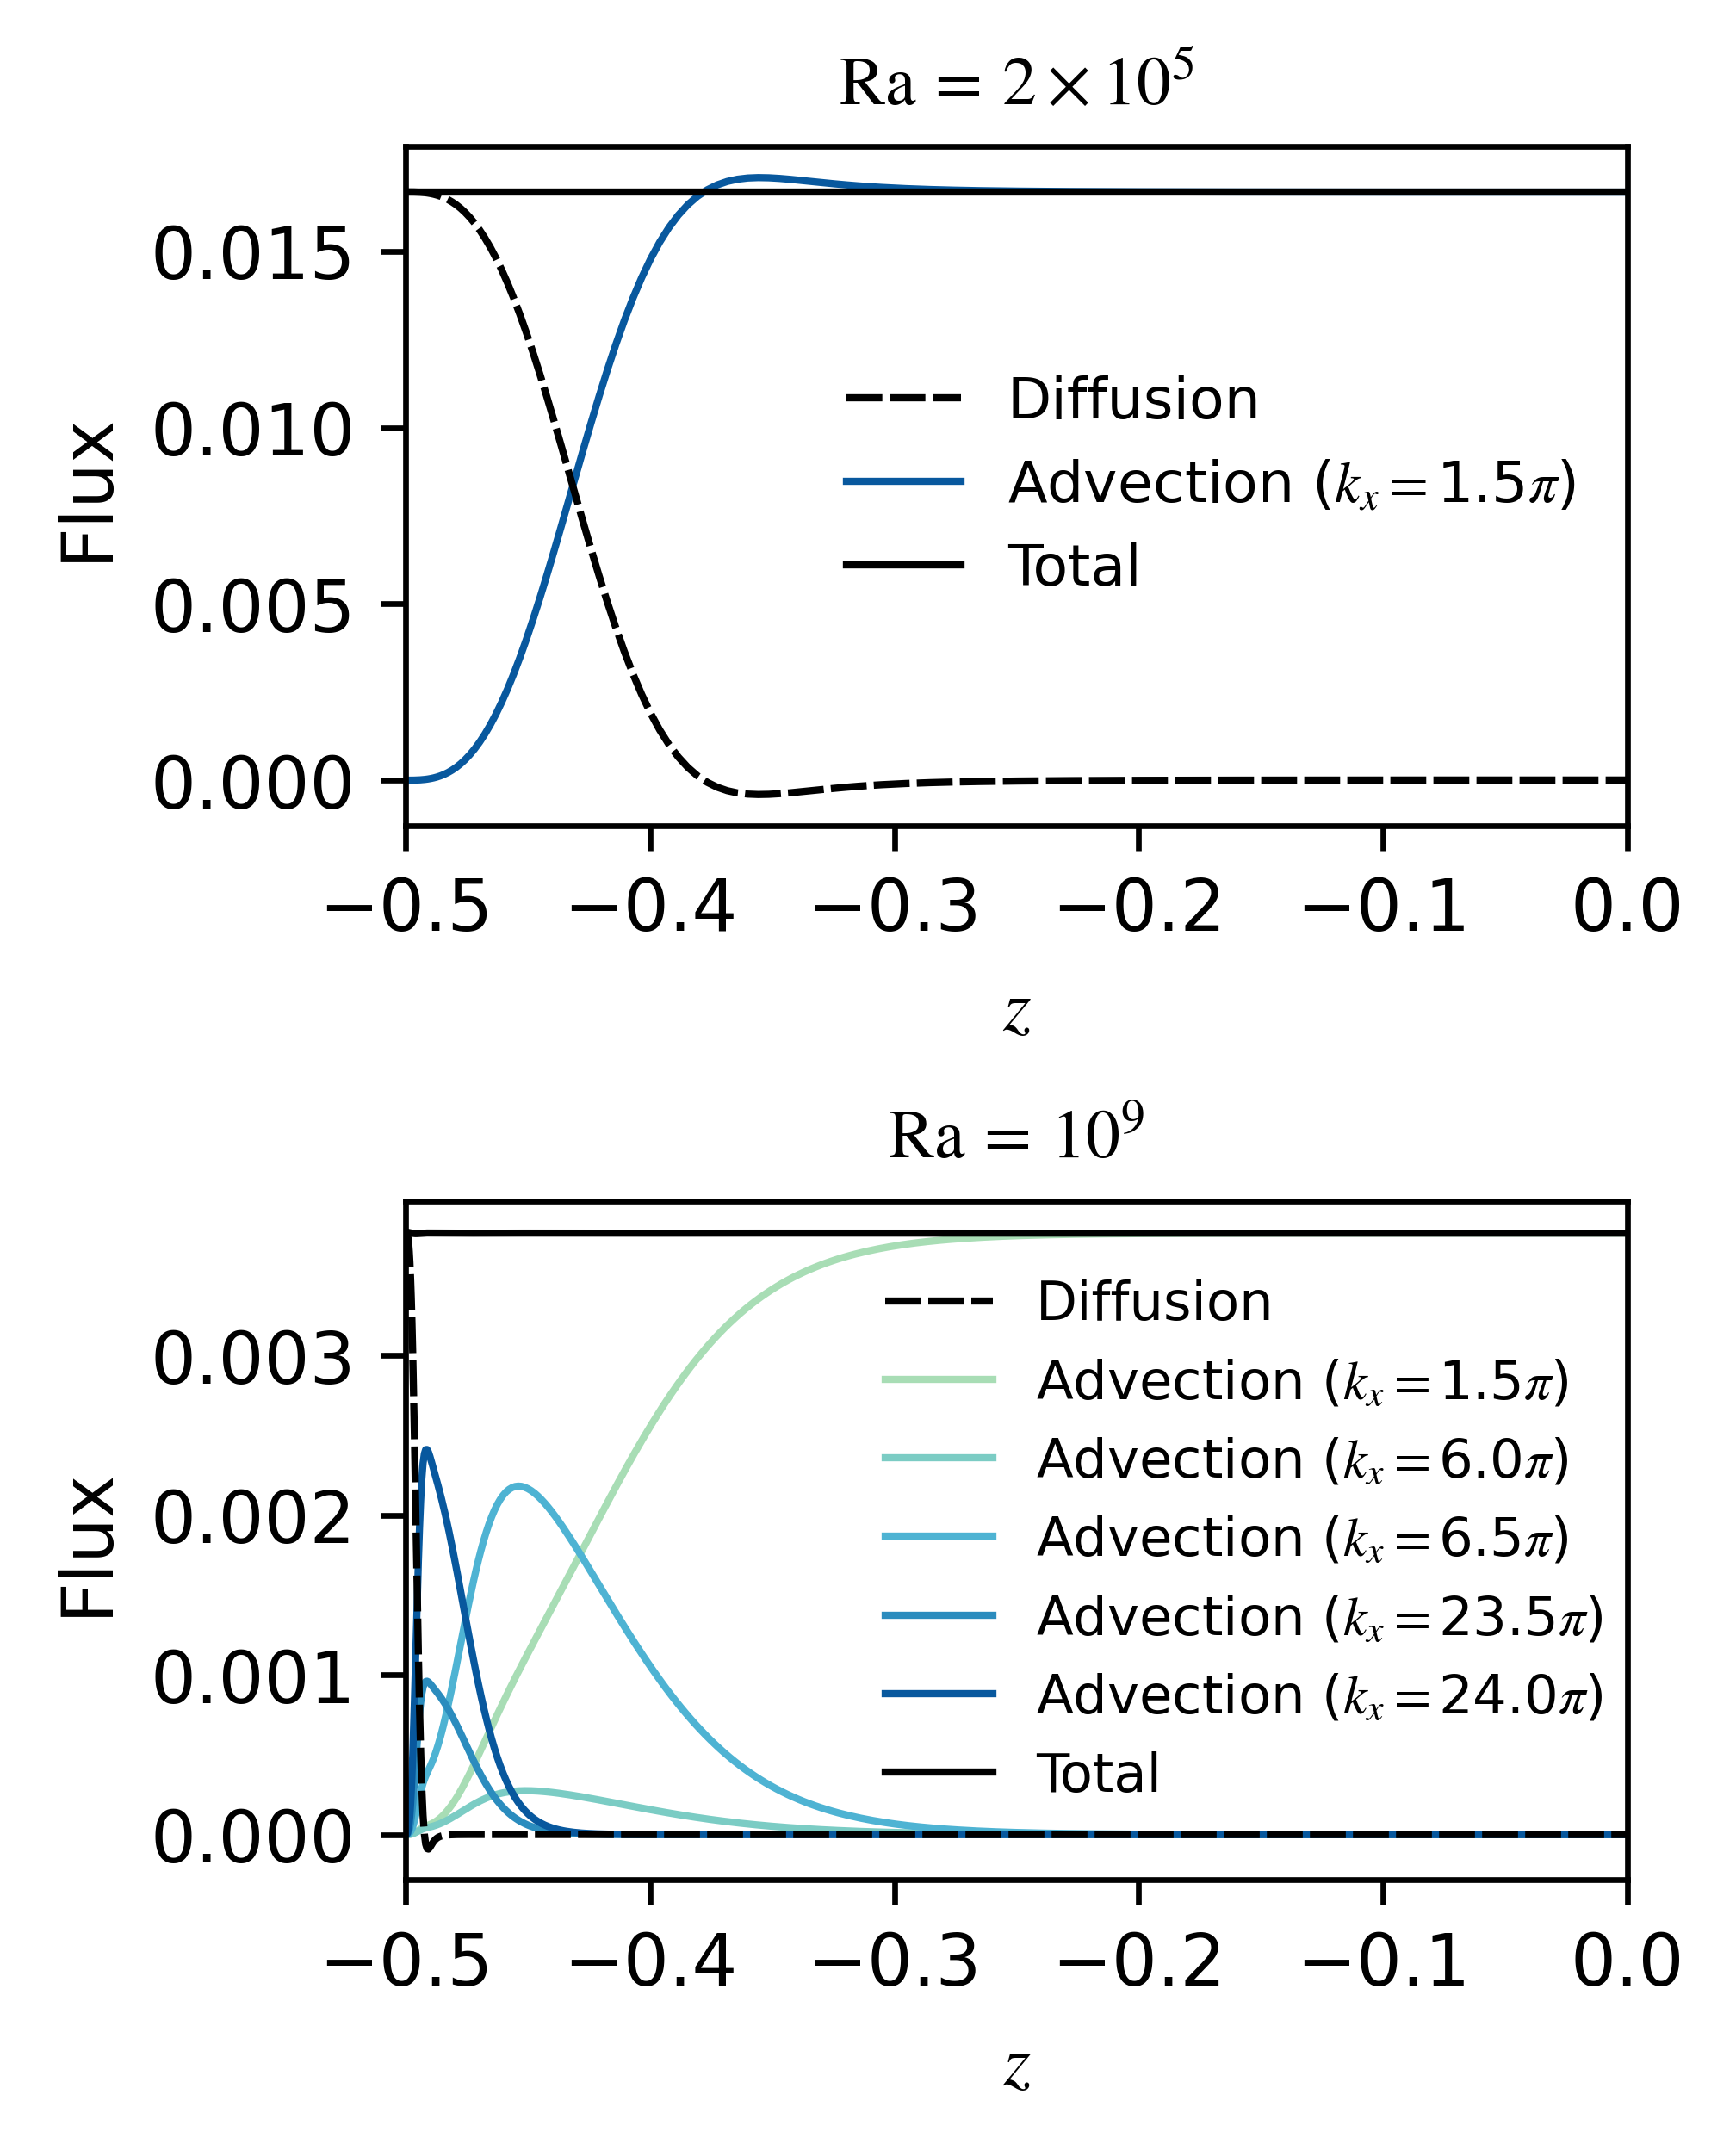
\includegraphics[width=3.4in]{flux_sup_n.png}}
    \subfloat{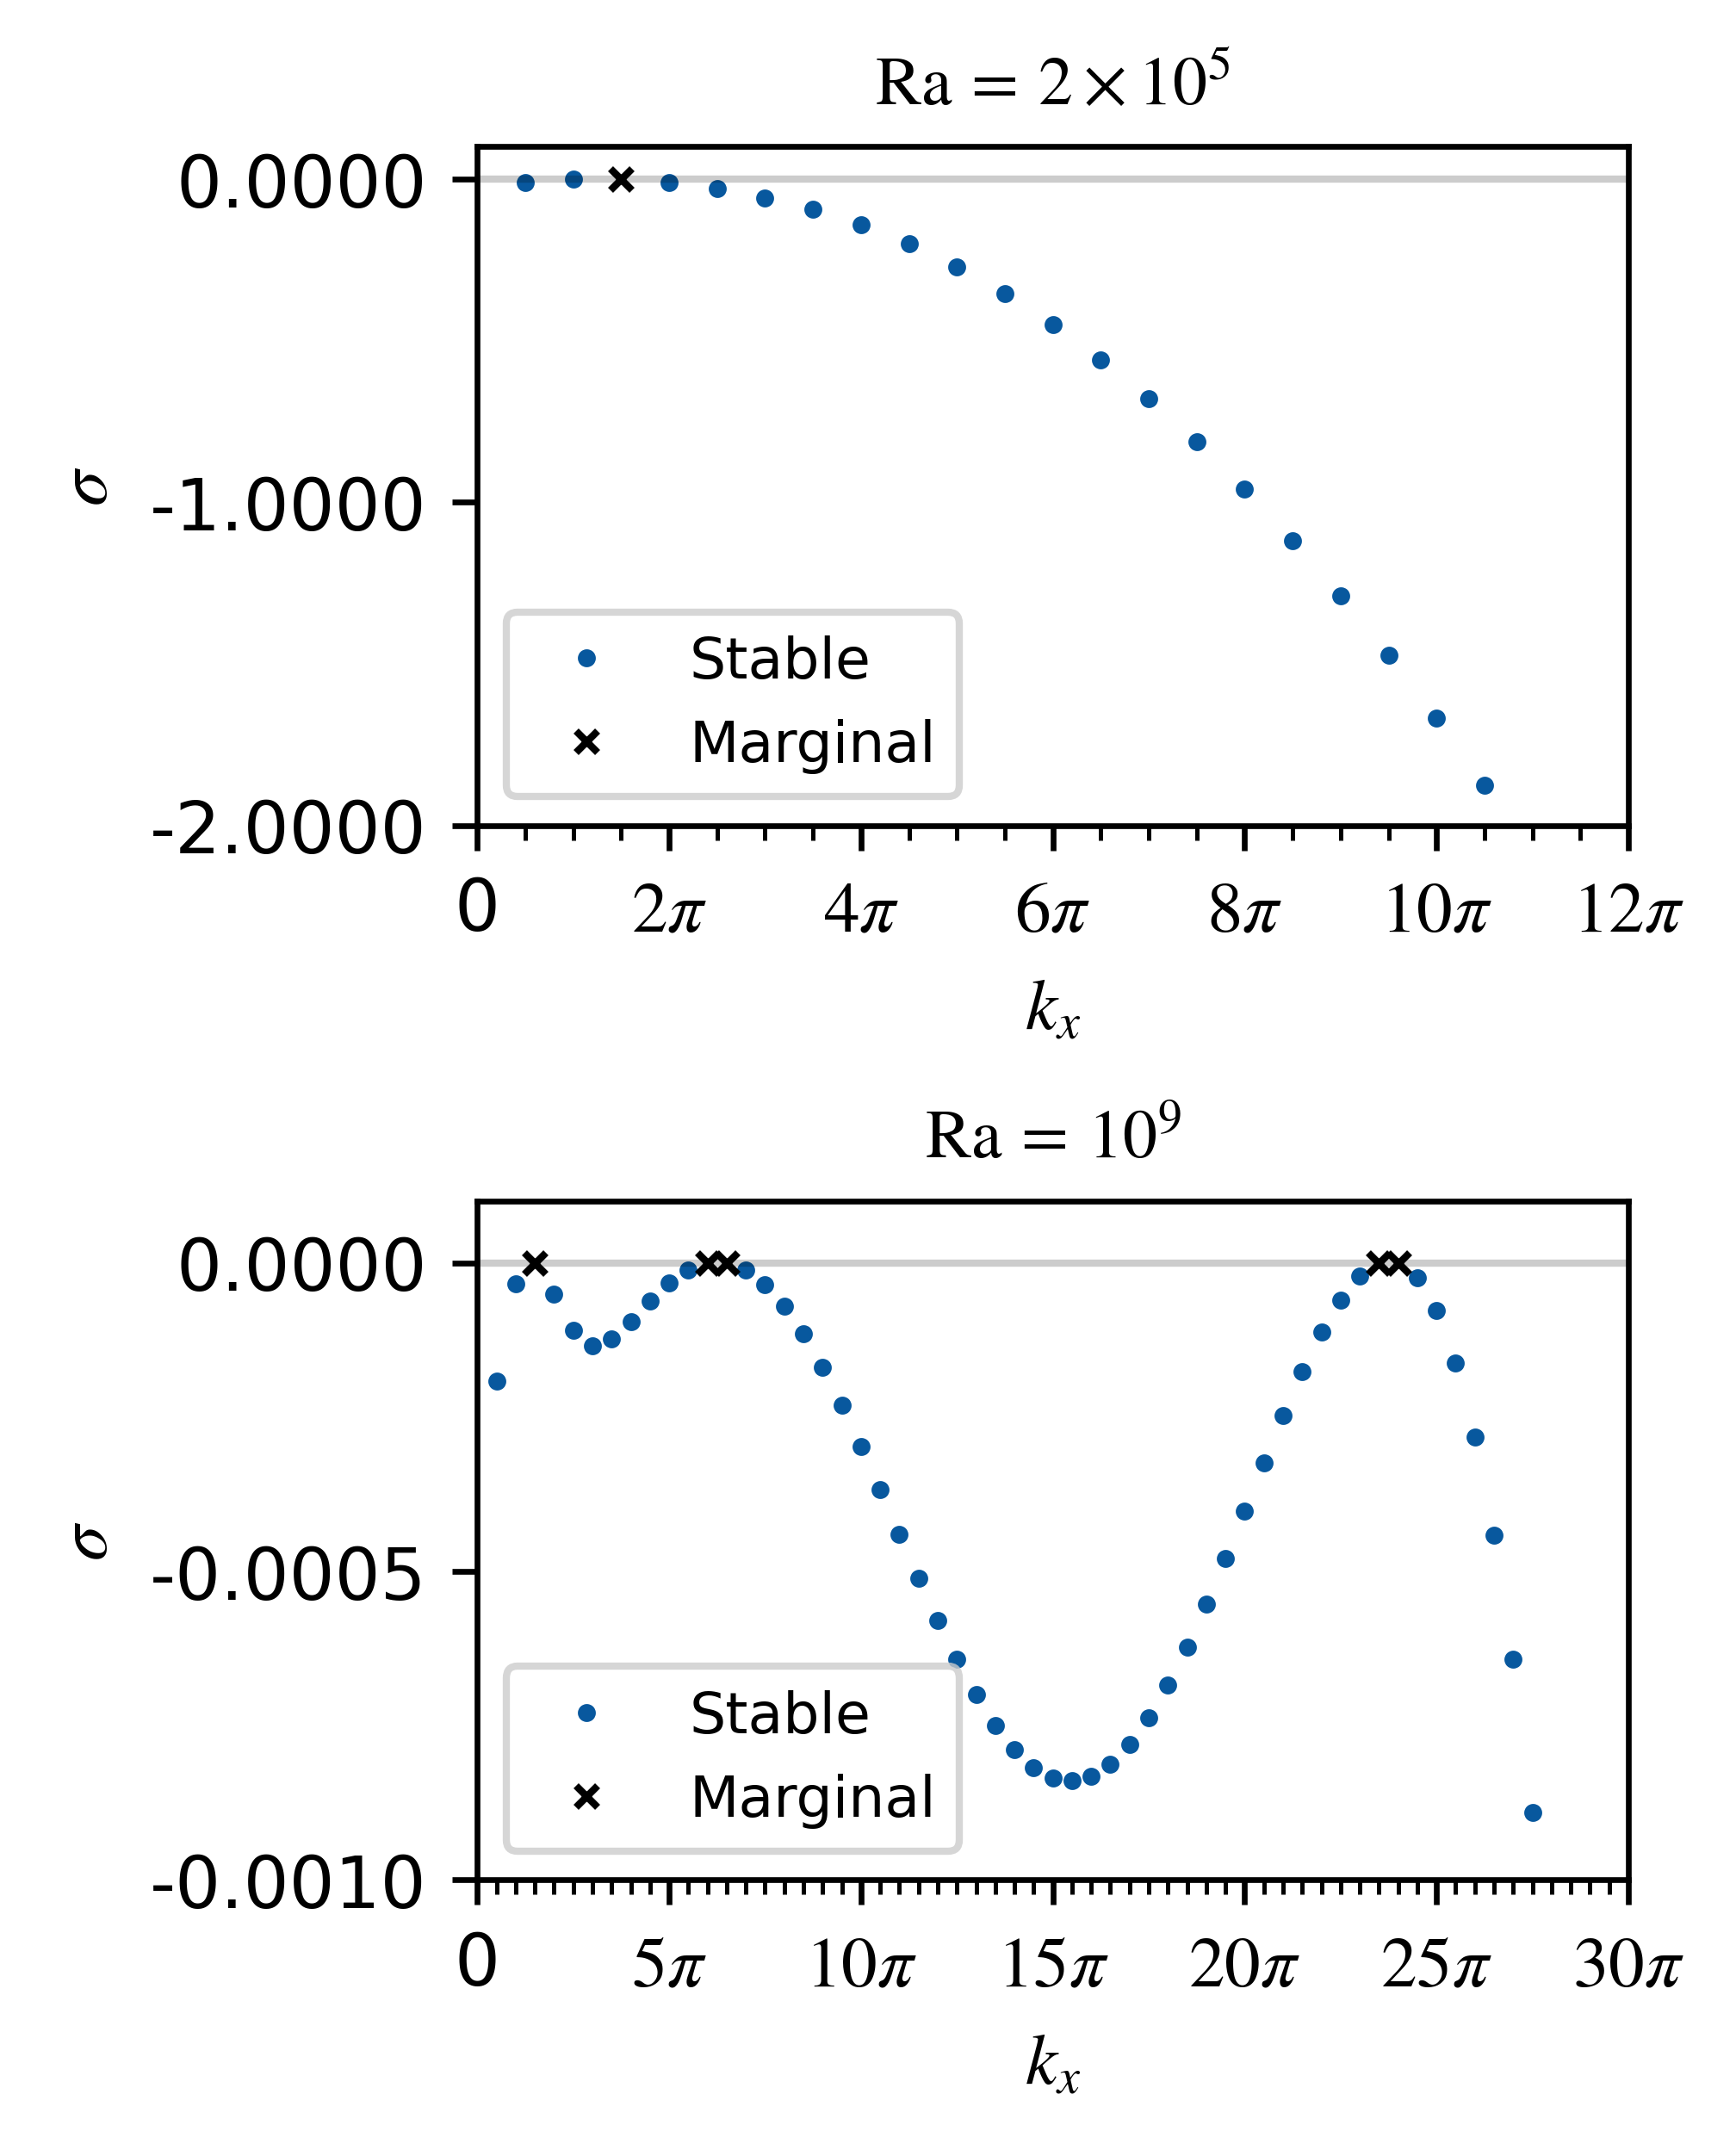
\includegraphics[width=3.4in]{EV_spectra_2ra.png}}
    \caption{Heat fluxes (left) and eigenvalue spectra (right) of equilibrated states $Ra = 2 \times 10^5$ (top) and $Ra = 10^9$ (bottom). Advection profiles belong to marginally-stable modes. For low $Ra$ a single mode with $k_x = 1.5\pi$ is sufficient to oppose  boundary layer diffusion and facilitate heat flux throughout the bulk of the domain. For large $Ra$, high-wavenumber marginally-stable modes contribute small-scale advection profiles which tightly hug the thin boundary layers. A combination of these of profiles is necessary to transition to the $k_x = 1.5\pi$ mode.}
    \label{fig:flux}
\end{figure*}

Equilibrated states exhibit distinct behaviors for large and small $Ra$. This contrast is well illustrated in Figure \ref{fig:flux}, where we give heat flux profiles and eigenvalue spectra for two cases: $Ra = 2 \times 10^5$ and $Ra = 10^9$. For lower $Ra$, there is a single presumed local maximum in the eigenvalue spectrum, whose adjacent modes' advection profiles occupy the bulk of the domain. Accordingly, these states have relaxed boundary regions which gradually diminish as the advection becomes the dominant component of the total flux. These transitional regions do not appear in the high $Ra$ cases, where the shift from diffusion to advection is sharp, requiring small-scale advection profiles belonging to modes adjacent to the third presumed local maximum in the eigenvalue spectrum. Traversing towards the midplane of the domain, we see increasingly thicker advection profiles corresponding the wavenumbers adjacent to the second local maximum, eventually culminating in the dominant $k_x = 1.5\pi$ mode.

\par The most resilient and unexpected feature of the associated background temperature profiles are the pronounced dips adjacent to the boundary layers. These dips appear in every solution, regardless of $Ra$. Physically, they correspond to thin layers in which the temperature gradient reverses. This counter-diffusion, which opposes the overall heat transfer, is overcome by the coinciding advective flux. High-wavenumber modes with large amplitudes oppose the intense diffusion by facilitating heat transfer towards the bulk of the domain via progressively lower wavenumber modes. In this bulk region, the $k_x = 1.5\pi$ mode is dominant regardless of $Ra$, suggesting that this mode is particularly important for systems of this kind. In the lower Rayleigh number cases, high-wavenumber modes are stable. The boundary layers and advective fluxes are relaxed, achieving equilibrium via a gradual transition from diffusion to advection.

% symmetry; batman ears; Nusselt number, BL thickness, and marginal kx's wrt Ra; flux figures w/ corresponding EV spectra; 
\begin{figure}[h]
    \centering
    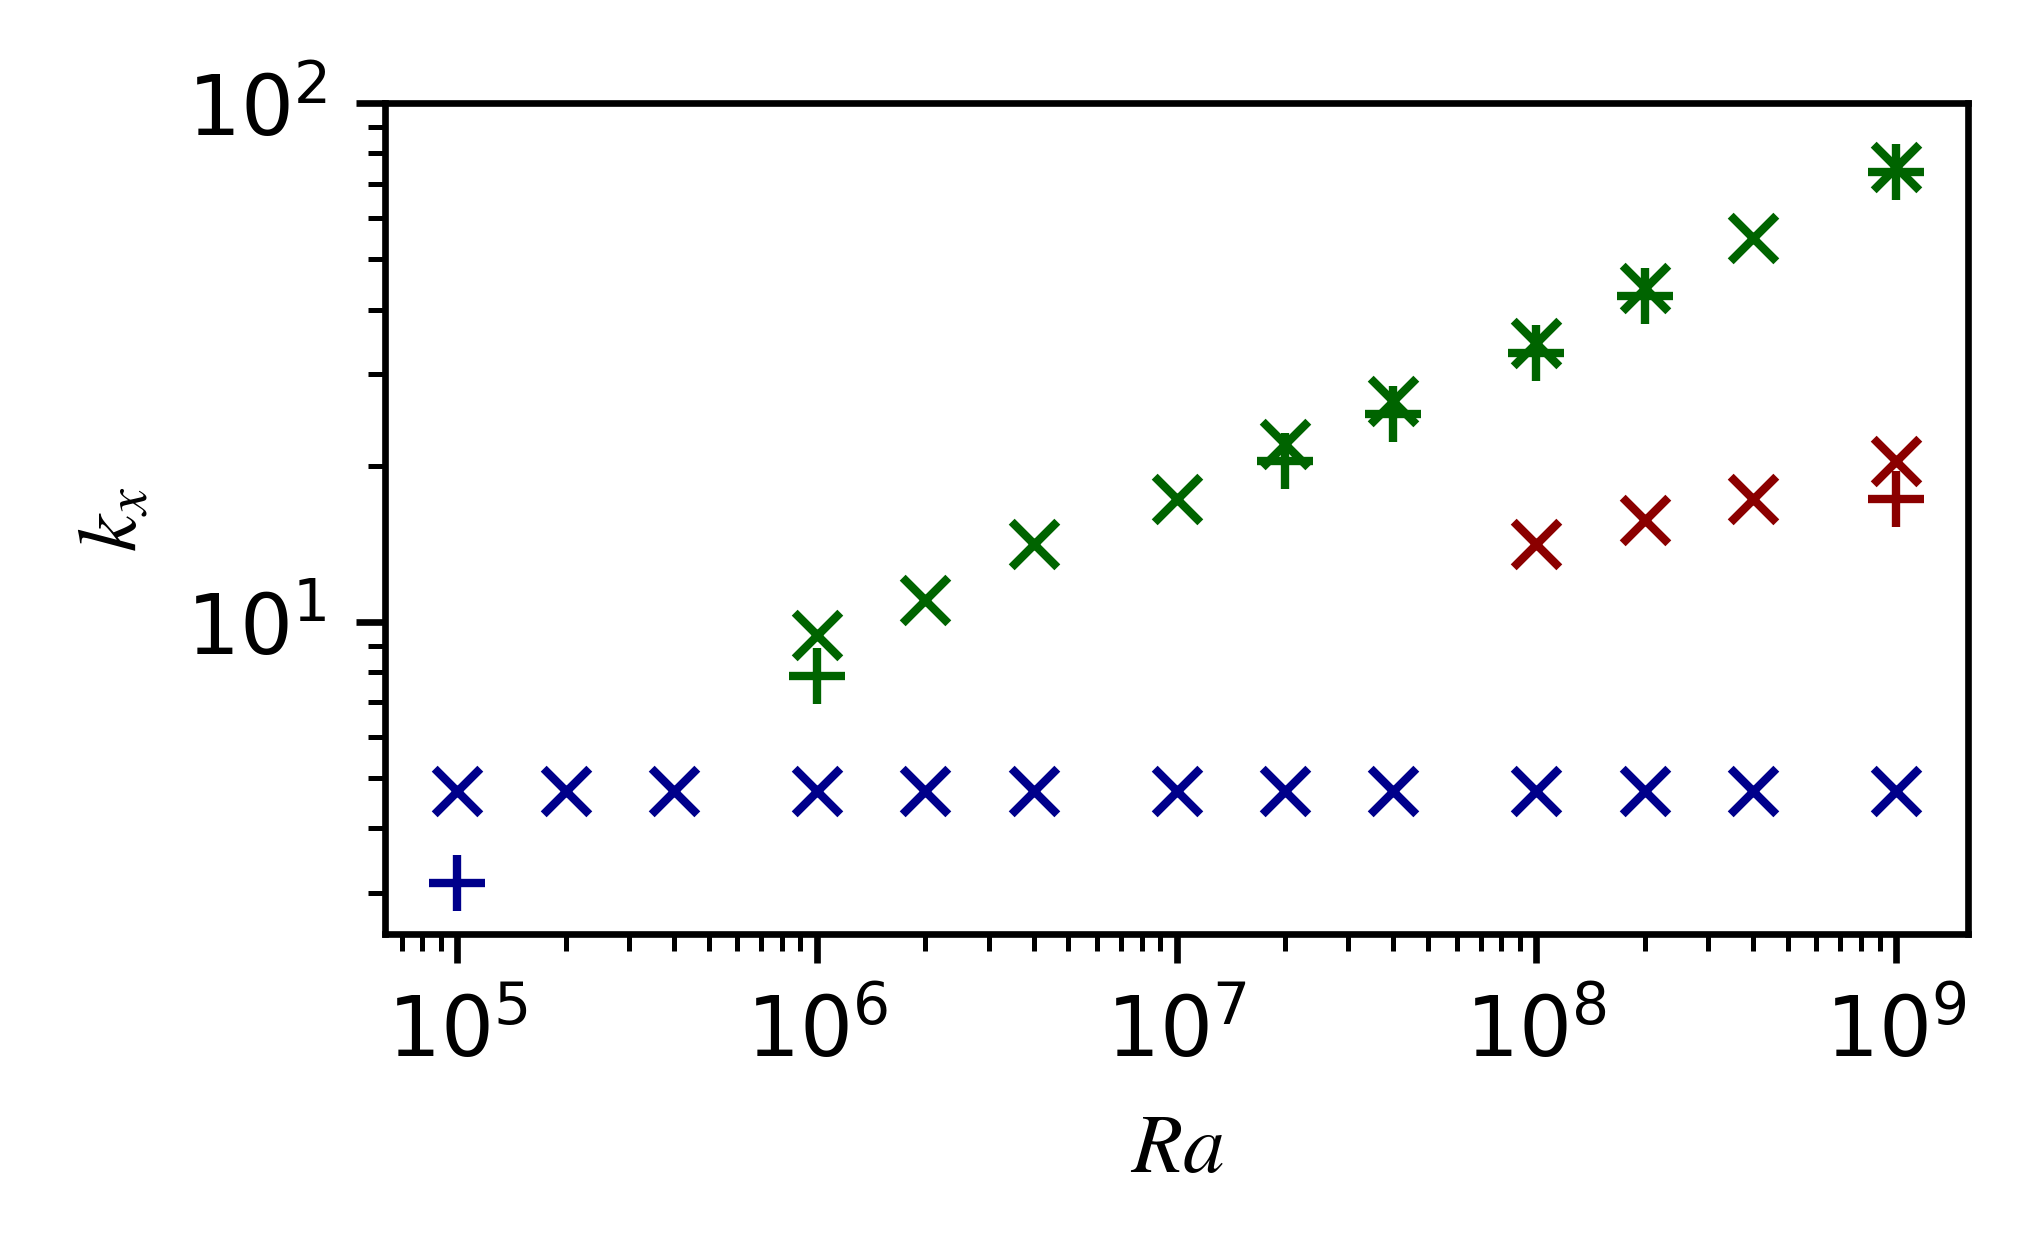
\includegraphics[width=3.4in]{kx_m_ra1.png}
    \caption{Wavenumbers of marginally-stable modes of thermally equilibrated states. Markers are color-coded according to their adjacent local maxima index in the eigenvalue spectrum. For example, the spectrum corresponding to $Ra = 10^5$ has marginal wavenumbers $k_x = \pi, \, 1.5\pi$ adjacent to a presumed local maximum between these two allowed values. The $Ra = 10^9$ spectrum, shown in lower right corner of Figure \ref{fig:flux}, has three presumed local maxima, with a single marginal mode adjacent to the first maximum ($k_x = 1.5\pi$), two marginal modes adjacent to the second maximum ($k_x = 6\pi, \, 6.5\pi$), and two marginal modes adjacent to the third maximum ($k_x = 23.5\pi, \, 24\pi$). The largest wavenumbers of the green branch obey a power-law relationship with $Ra$}
    \label{fig:kx_marginals}
\end{figure}






\begin{figure}[h]
    \centering
    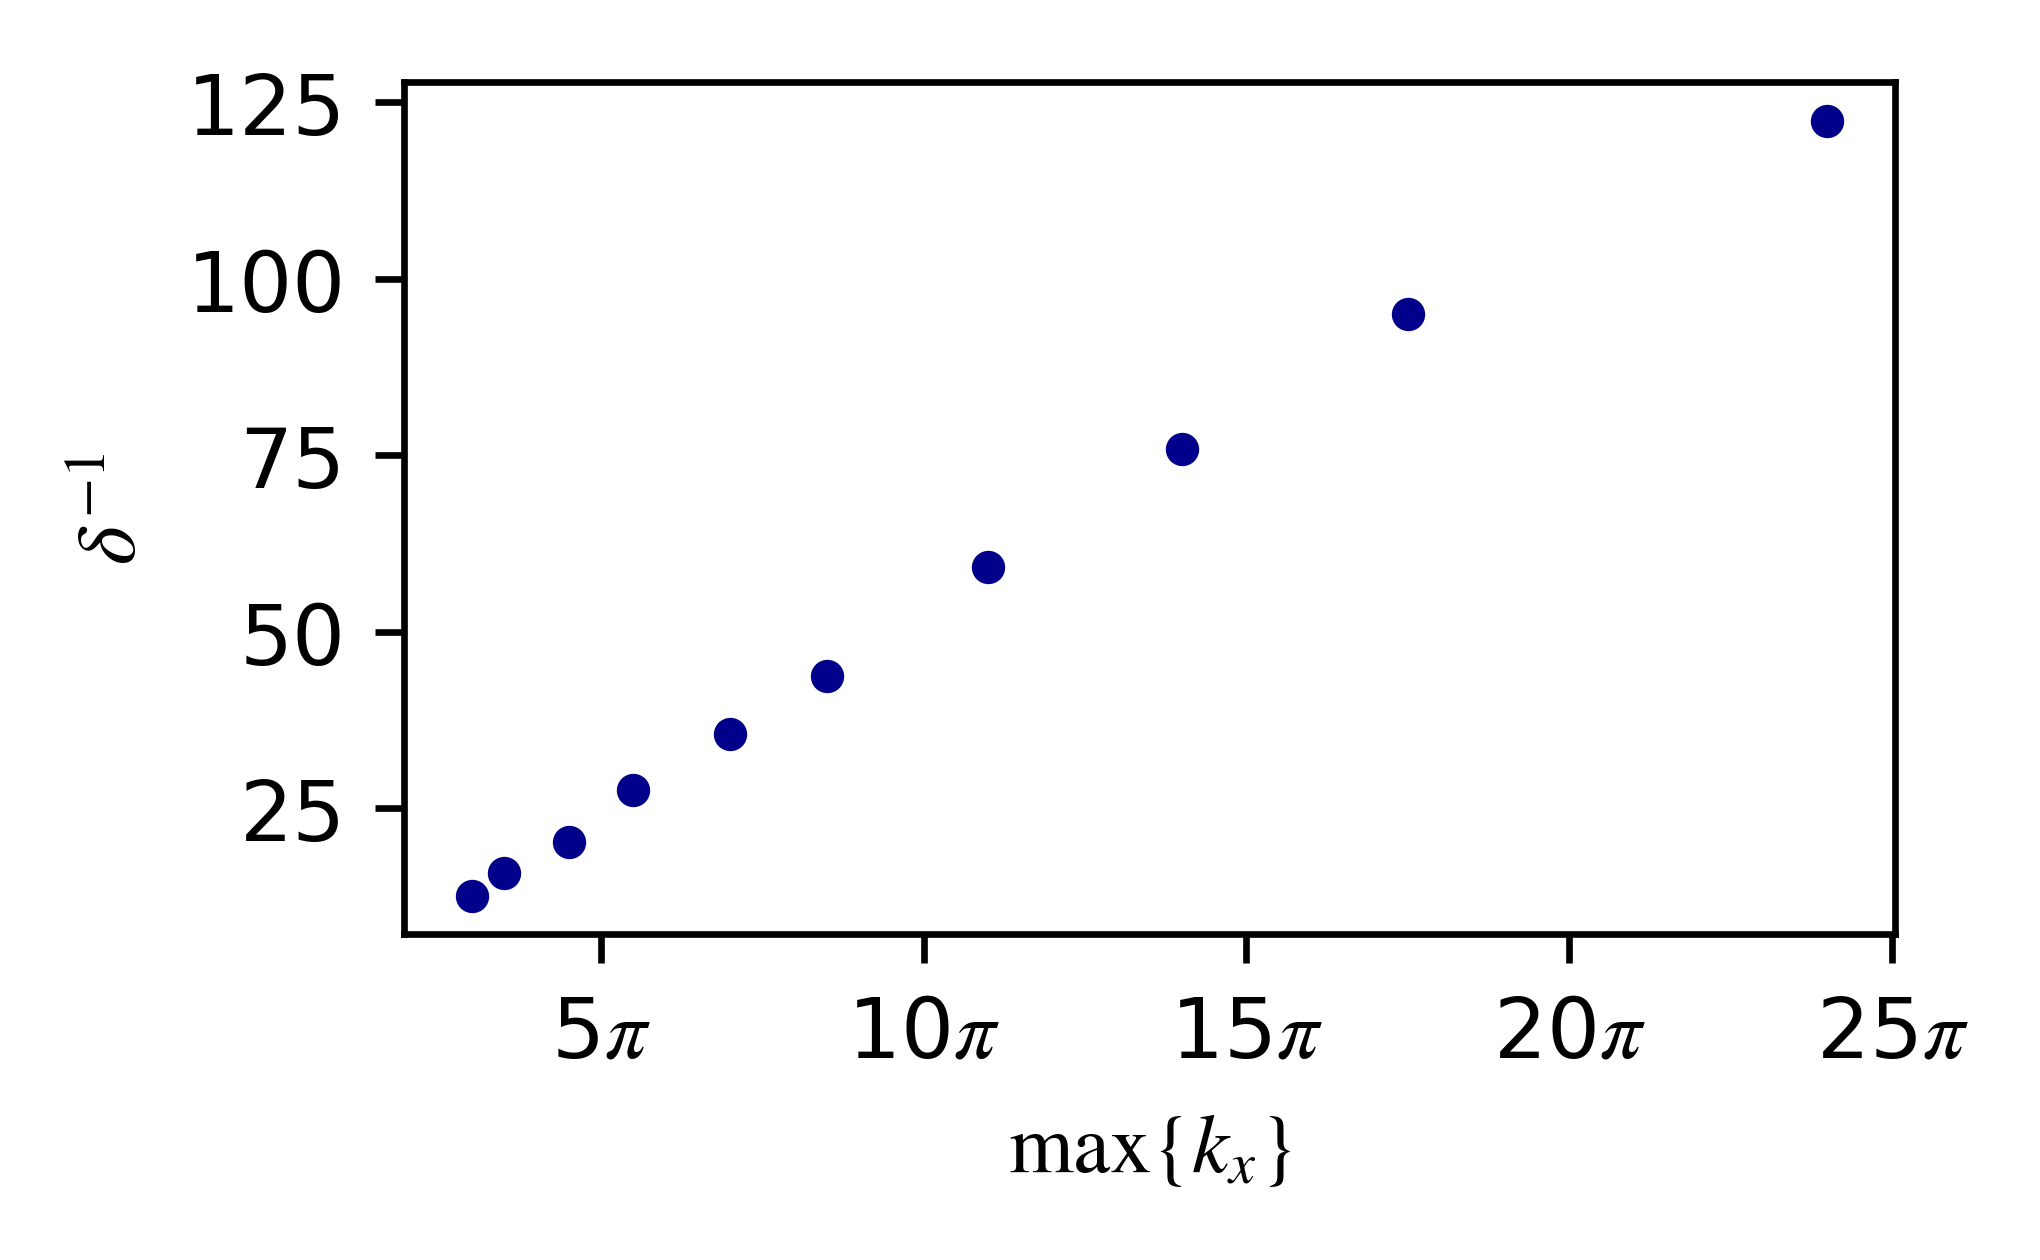
\includegraphics[width=3.4in]{del_kx_inv.png}
    \caption{For $Ra \geq 10^6$, the maximum marginally-stable wavenumber (corresponding to the green X markers in Figure \ref{fig:kx_marginals}) are inversely related to the boundary layer thicknesses $\delta$. $\max \{ k_x \}$ gives a minimum $x$ length scale for the perturbations, and consequently, the advection. We expect the minimum $z$ length scale to agree with the boundary layer thickness $\delta$ because otherwise the boundary layer would continue to diffuse. This is well illustrated in the lower left corner of Figure \ref{fig:flux}, where the advection profile for $k_x = 24\pi$ is tightly flanked by the surrounding boundary layers. This suggests that the minimum $x$ and $z$ length scales obey some constant ratio.}
    \label{fig:my_label}
\end{figure}

\begin{figure*}[h]
    \centering
    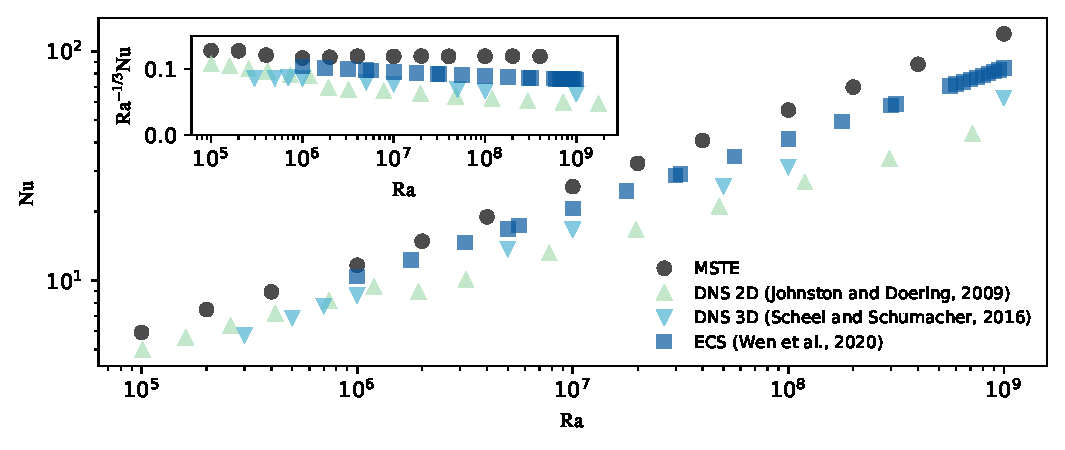
\includegraphics[width=7.1in]{nu_ra.PNG}
    \caption{Nusselt number of iterative marginal convection solutions.}
    \label{fig:nu_vs_ra}
\end{figure*}
\begin{figure}[h]
    \centering
    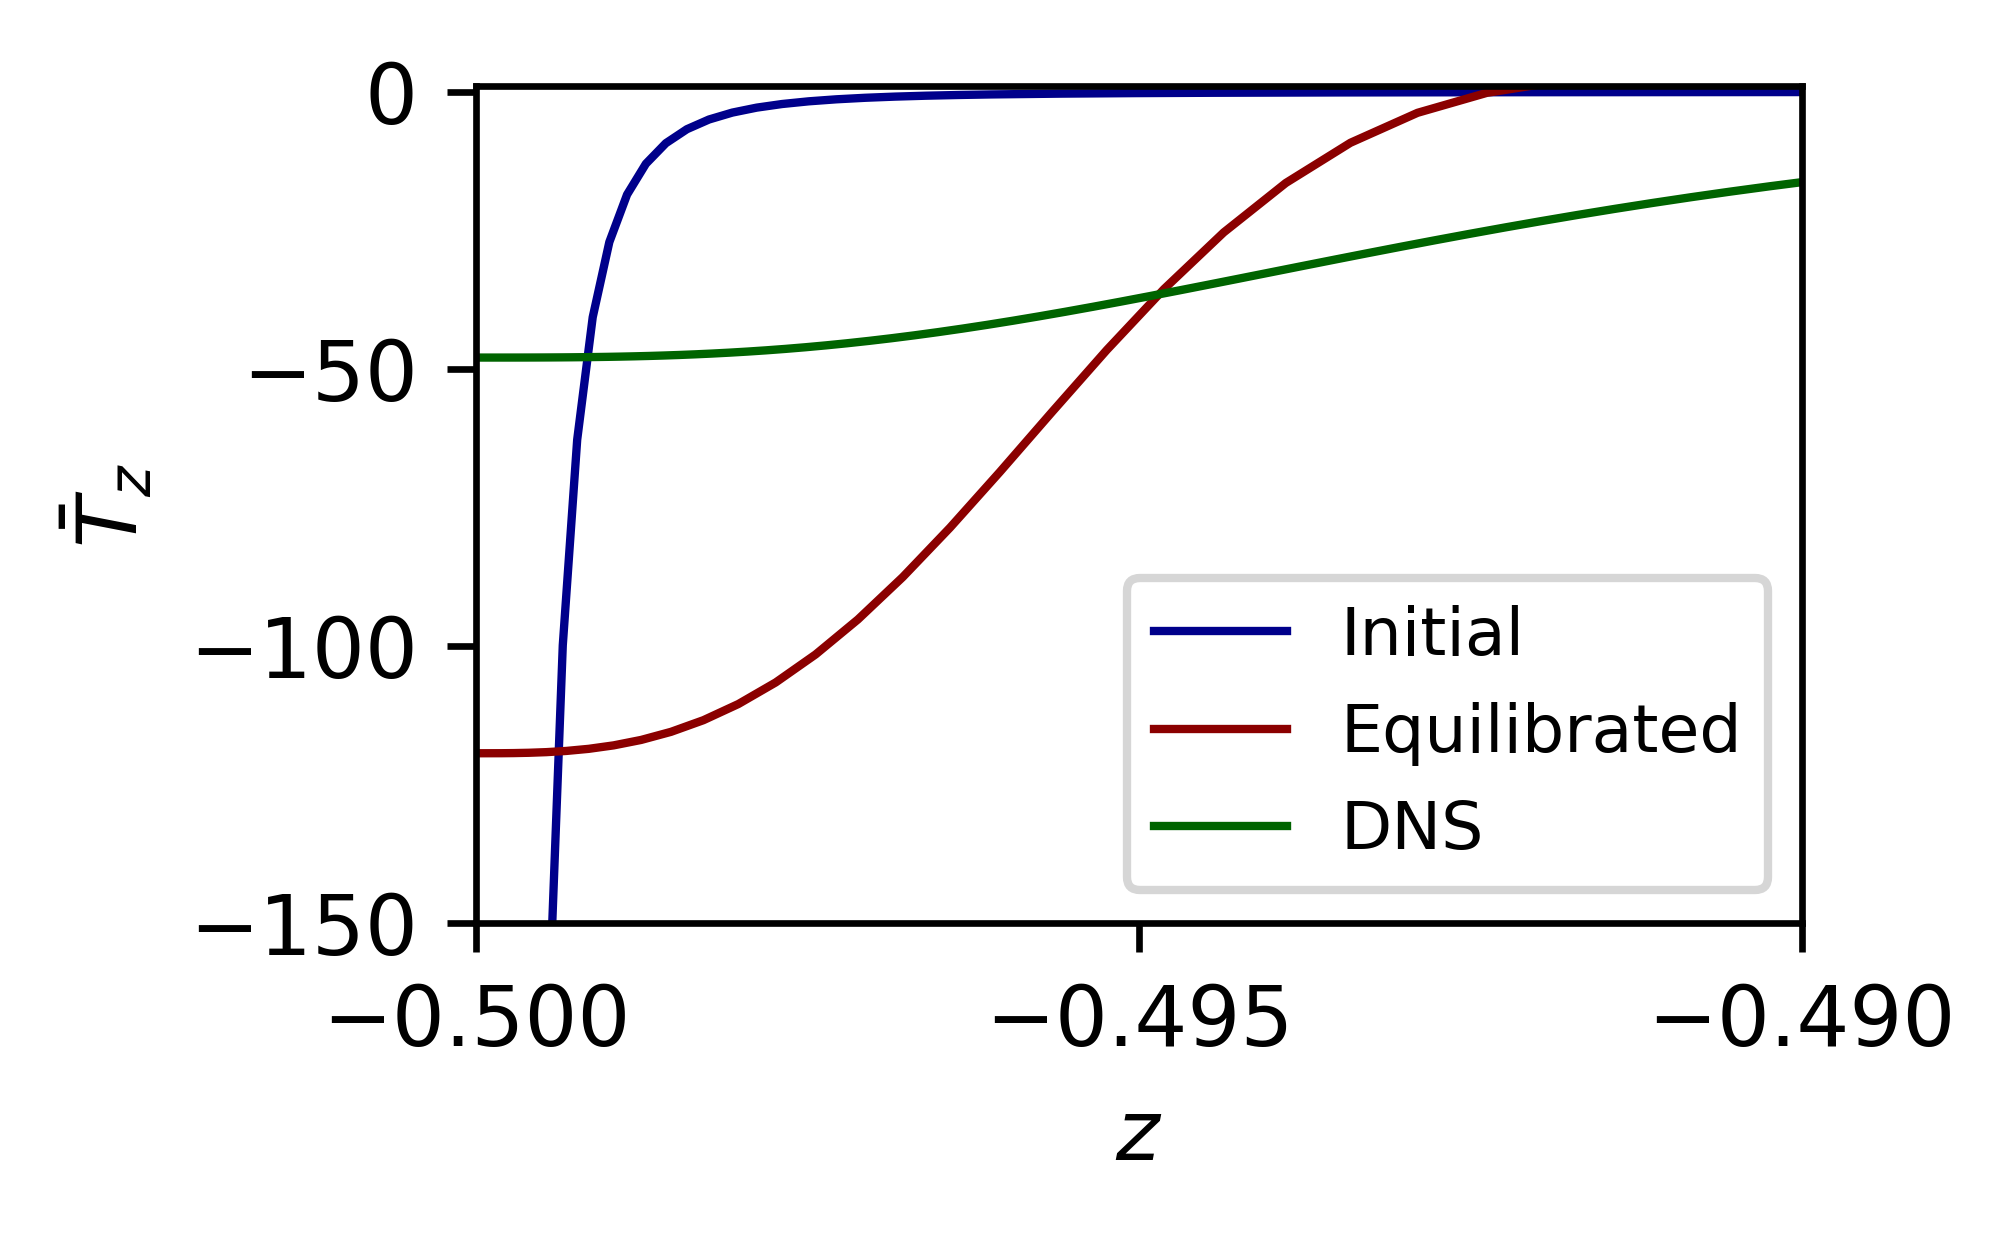
\includegraphics[width=3.4in]{b0z_profs.png}
    \caption{Background temperature profiles.}
    \label{fig:my_label}
\end{figure}

% \begin{figure}[h]
%     \centering
%     \includegraphics[width=3.4in]{wb_profiles_norm.png}
%     \caption{Horizontally-averaged advective flux}
%     \label{fig:my_label}
% \end{figure}
 \newpage
\section{Simulations with Thermally Equilibrated Initial Conditions}

\begin{figure}[h]
    \centering
    \includegraphics[width=3.4in]{nu_good.png}
    \caption{Simulation Nusselt number: 2-dimensional nonlinear simulations were performed with identical parameters.}
    \label{fig:my_label}
\end{figure}

\begin{figure}[h]
    \centering
    \includegraphics[width=3.4in]{ke_good.png}
    \caption{Maximum simulation kinetic energy}
    \label{fig:my_label}
\end{figure}

% \begin{figure}[h]
%     \centering
%     \subfloat{\includegraphics[width=3.4in]{write_000001.png}}
%     \hfill
%     \subfloat{\includegraphics[width=3.4in]{write_000004.png}}
%     \caption{Quasi-geostrophic potential vorticity (PV) with an overwhelming beta-effect shown at time $t \approx 0.5$. Disco-ball initial conditions are employed. Left and right figures obtained from finite difference and \texttt{Dedalus} solvers respectively.} 
%     \label{beta}
% \end{figure}

\section{Conclusion}\label{sec:conclusion}

\section*{Appendix}
This is an appendix

\section*{Acknowledgments}
We thank the people of Ohio.

\bibliography{she}

\end{document}

